\subsection{Mid-Frequency Estimation} \label{sec:midfreqest}

\begin{frame} \frametitle{Mid-Frequency Estimation}
    \framesubtitle{Purpose}
    \begin{itemize}
        \item Specify contribution from carrier
            \begin{itemize}
                \item $\angle s(t) = \phi (t) + 2 \pi f_c t$
            \end{itemize}
    \end{itemize}
    \begin{center}
        \includegraphics[width=0.9\textwidth]{img/phase_carrier}
    \end{center}
\end{frame}

\begin{frame} \frametitle{Mid-Frequency Estimation}
    \framesubtitle{Properties}
    \begin{center}
        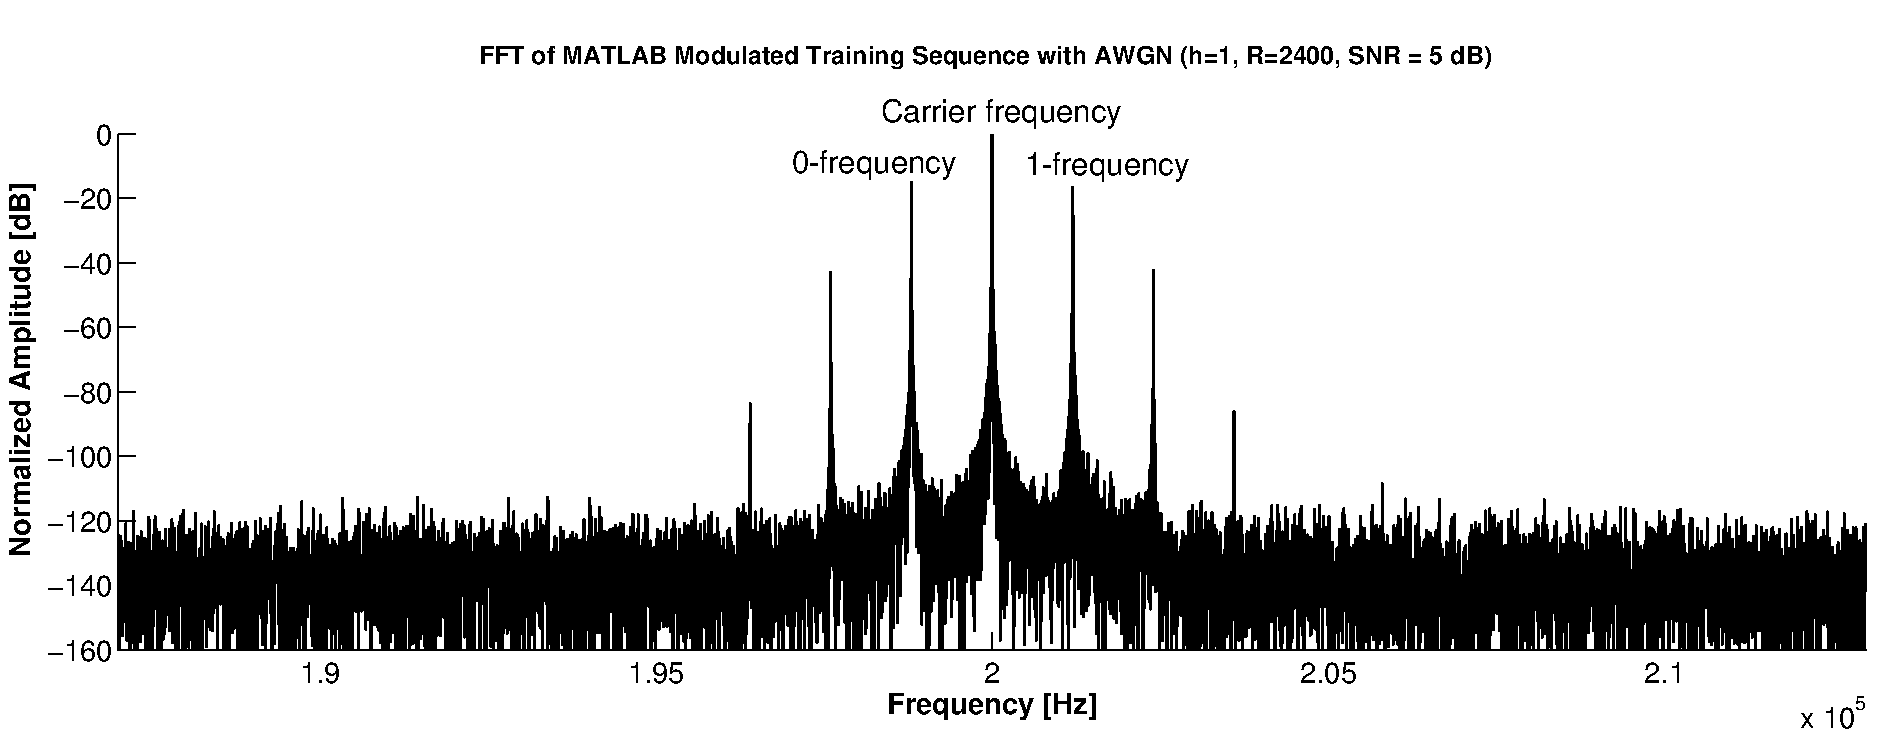
\includegraphics[width=1.0\textwidth]{img/fft_train_seq}
    \end{center}
    \begin{itemize}
        \item Performing an 8192-point FFT on the DSP
        \item 8192 samples are approximately 13 bytes of training sequence
        \begin{itemize}
            \item $f_s = \SI{758272}{Hz}$, $R = 9600$, $\texttt{SPS} \approx 79$
        \end{itemize}
    \end{itemize}
    \begin{center}
        \resizebox{9cm}{!}{
            \begin{tabular}{|c|c|c|c|c|}
                \hline
                $N$ [\si{samples}]          & $f_\text{res}$ [\si{Hz}]
                & FFT cycles [\si{kcycles}] & max cycles [\si{kcycles}]
                & $\text{FFT usage}$ [\si{\%}]\\ \hline
                8192 & 92.6 & 213  & 142.433 & 0.150\\ \hline
            \end{tabular}
        }
    \end{center}
\end{frame}

\begin{frame} \frametitle{Mid-Frequency Estimation}
    \framesubtitle{Test Results}
    Tested with signal generator.
    \begin{center}
        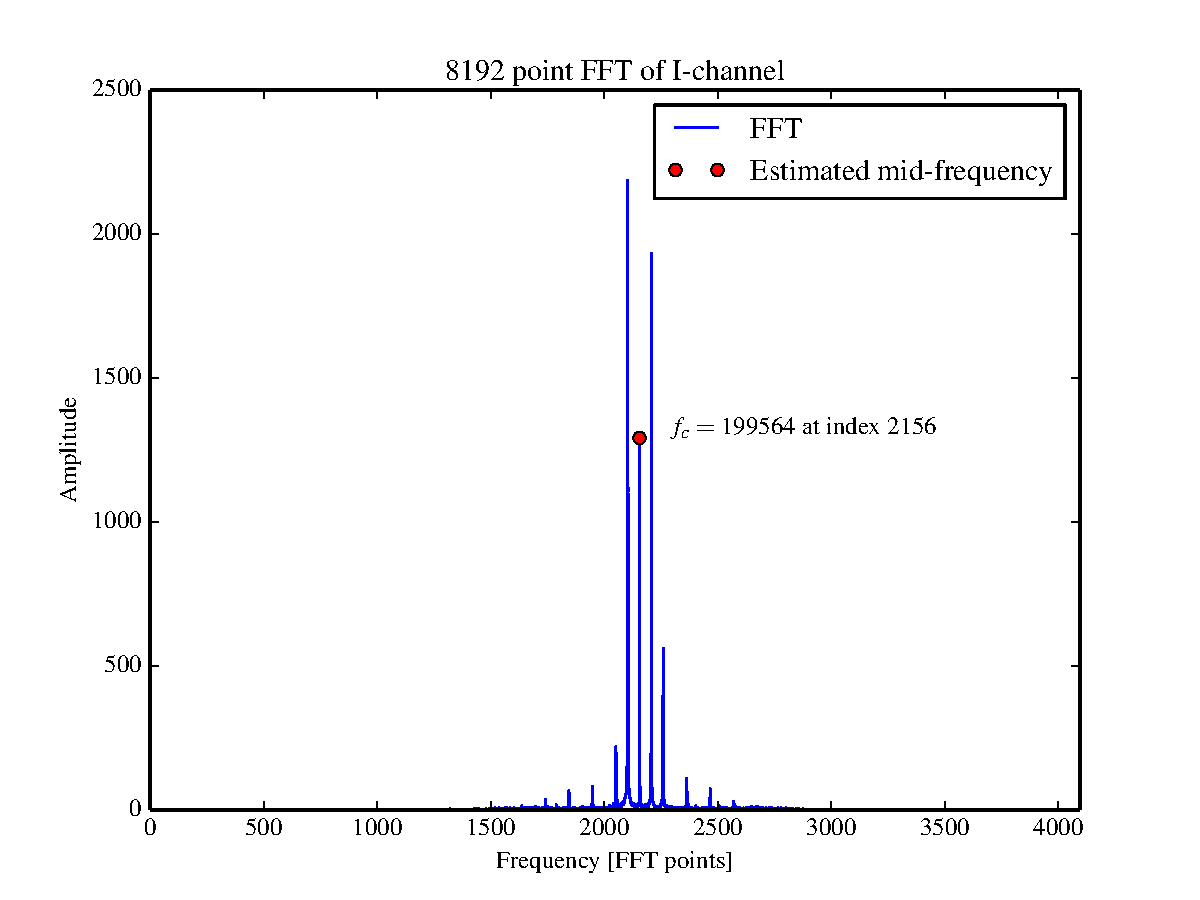
\includegraphics[width=0.7\textwidth]{img/fft_dsp}
    \end{center}
    \begin{itemize}
        \item Actual mid-frequency
            \begin{itemize}
                \item $\SI{199567}{Hz}$
            \end{itemize}
        \item Estimated mid-frequency
            \begin{itemize}
                \item $\SI{199564}{Hz}$
            \end{itemize}
    \end{itemize}
\end{frame}


\subsection{Time Synchronization} \label{sec:finaltest}

\begin{frame} \frametitle{Time Synchronization}
    \framesubtitle{Purpose}
    \begin{itemize}
        \item Timing is needed to decide the value of each symbol
    \end{itemize}
    \begin{center}
        \vspace{1cm}
        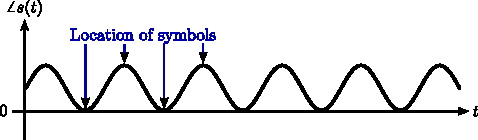
\includegraphics[width=0.9\textwidth]{img/time_sync_purp}
    \end{center}
\end{frame}

\begin{frame} \frametitle{Time Synchronization}
    \framesubtitle{Frequency translation}
    \definecolor{mikred}{RGB}{170,0,0}
    \definecolor{mikblue}{RGB}{0,0,170}
    \begin{itemize}
        \item The downconverted phase-signal is used for time synchronization
        \item \textcolor{mikred}{The phase-signal is computed}
        \item \textcolor{mikblue}{The slope added by the carrier and Doppler shift is subtracted}
            \begin{itemize}
                \item \textcolor{mikred}{$\angle s(t) =$} $\phi (t)$ \textcolor{mikblue}{$+ 2 \pi f_{c,est} t$}
            \end{itemize}
    \end{itemize}
    \begin{center}
        \includegraphics[width=0.9\textwidth]{img/phase_carrier}
    \end{center}
\end{frame}

\begin{frame}
    \frametitle{Time Synchronization}
    \framesubtitle{Wrapping}
    \begin{center}
        \includegraphics{img/phaseslope}
    \end{center}
    \begin{itemize}
    \item Wrapping: $\mathtt{arg\_fr16(phi)} \in [-\pi,\pi)$, $\mathtt{fract16} \in [-2^{15},2^{15})$.
    \item Scale $\pi \equiv 2^{15}$ -- wraps around unit circle.
    \end{itemize}
\end{frame}

\begin{frame}
    \frametitle{Time Synchronization}
    \framesubtitle{Cross-Correlation}
    \begin{itemize}
        \item Cross-correlation of downconverted phase-signal, $y_2$, and pre-computed triangle wave, $y_1$
    \end{itemize}
    \begin{equation*}
        % \psi_{y_1y_2}(\tau) = \int_{-\infty}^{\infty} y_1(t)y_2(t+\tau) \mathrm{d} t
        \psi_{y_1y_2}[\tau] = \frac{1}{N}\sum_{n=0}^{N-2T_b-1} y_1[n]y_2[n+\tau], \quad \tau \in [0, \; 2T_b]
    \end{equation*}
    \begin{center}
        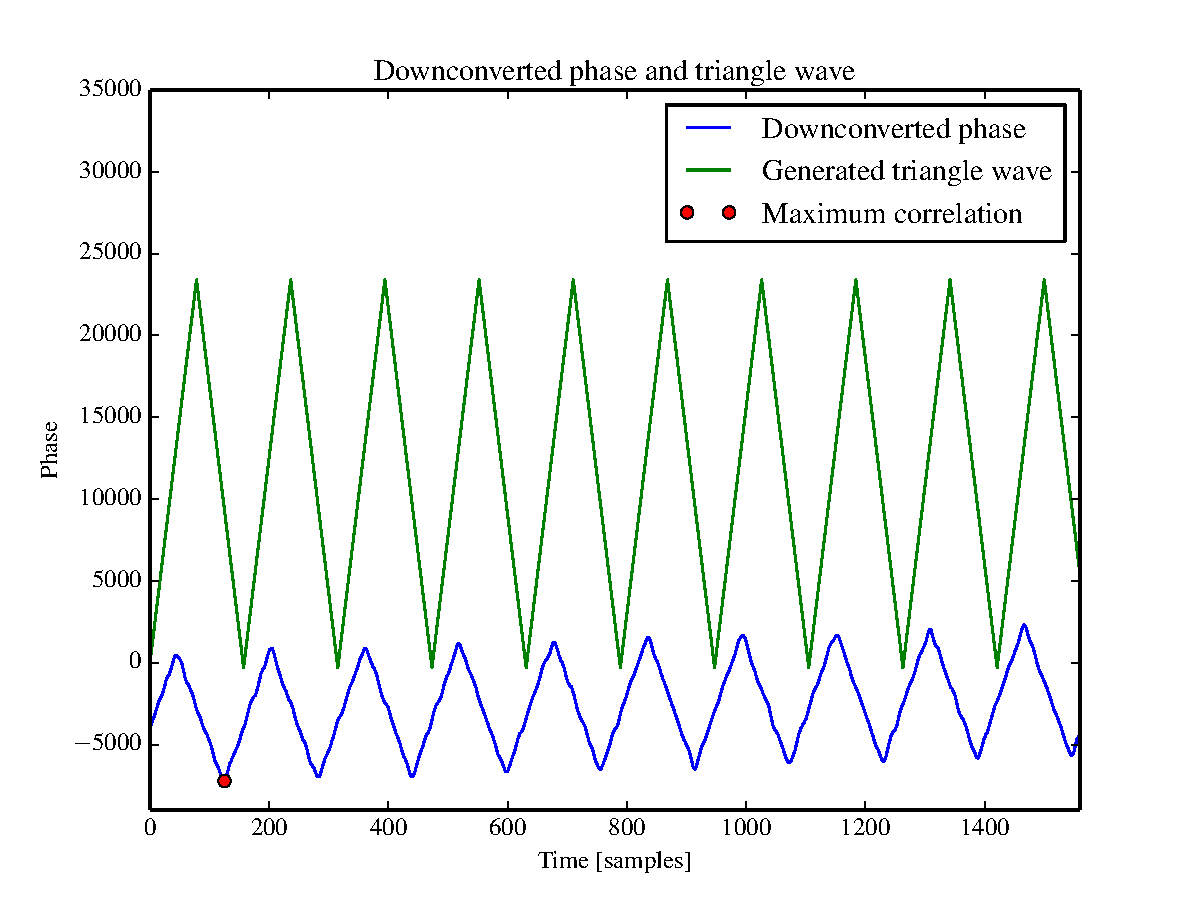
\includegraphics[width=0.5\textwidth]{img/phase_triang}
        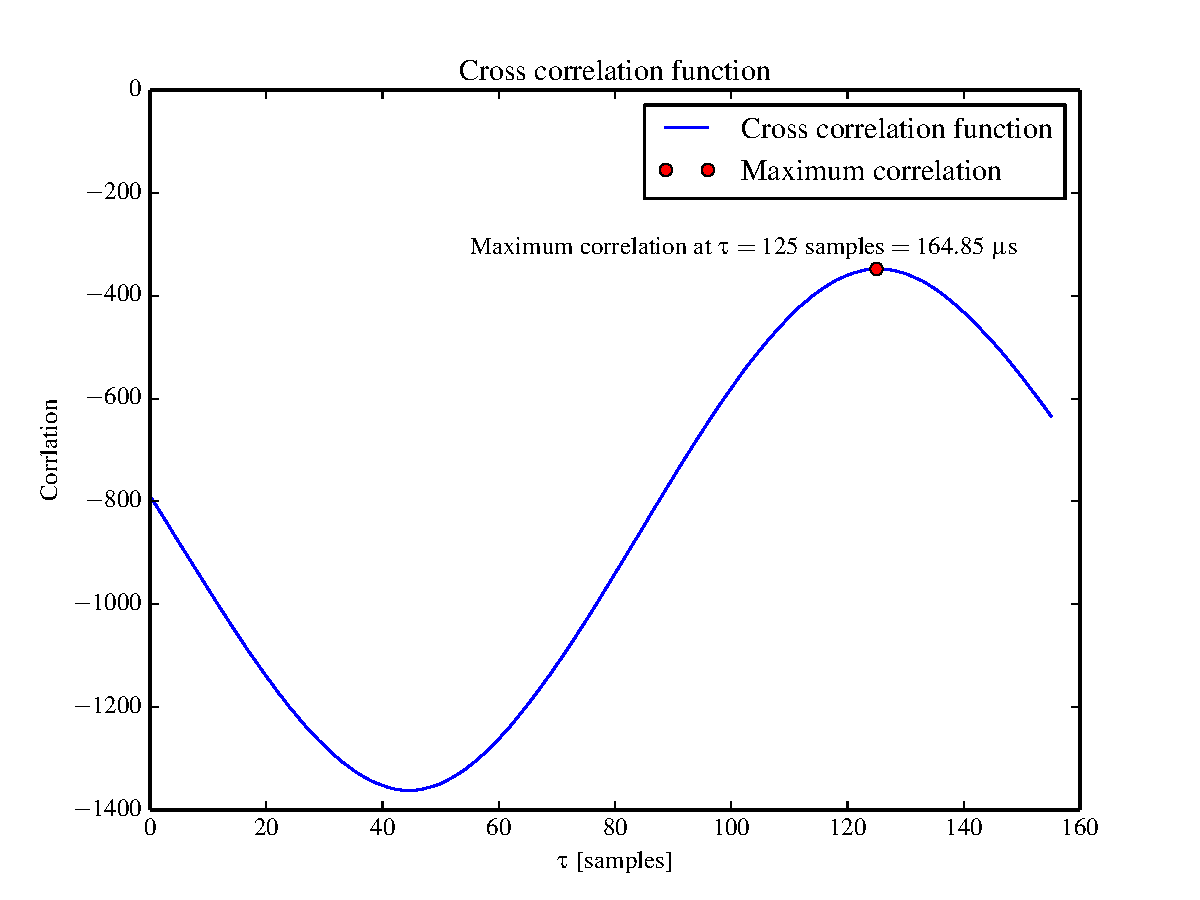
\includegraphics[width=0.5\textwidth]{img/crosscorr}
    \end{center}
\end{frame}

\begin{frame} \frametitle{Time Synchronization}
    \framesubtitle{Test Results}
    \begin{center}
        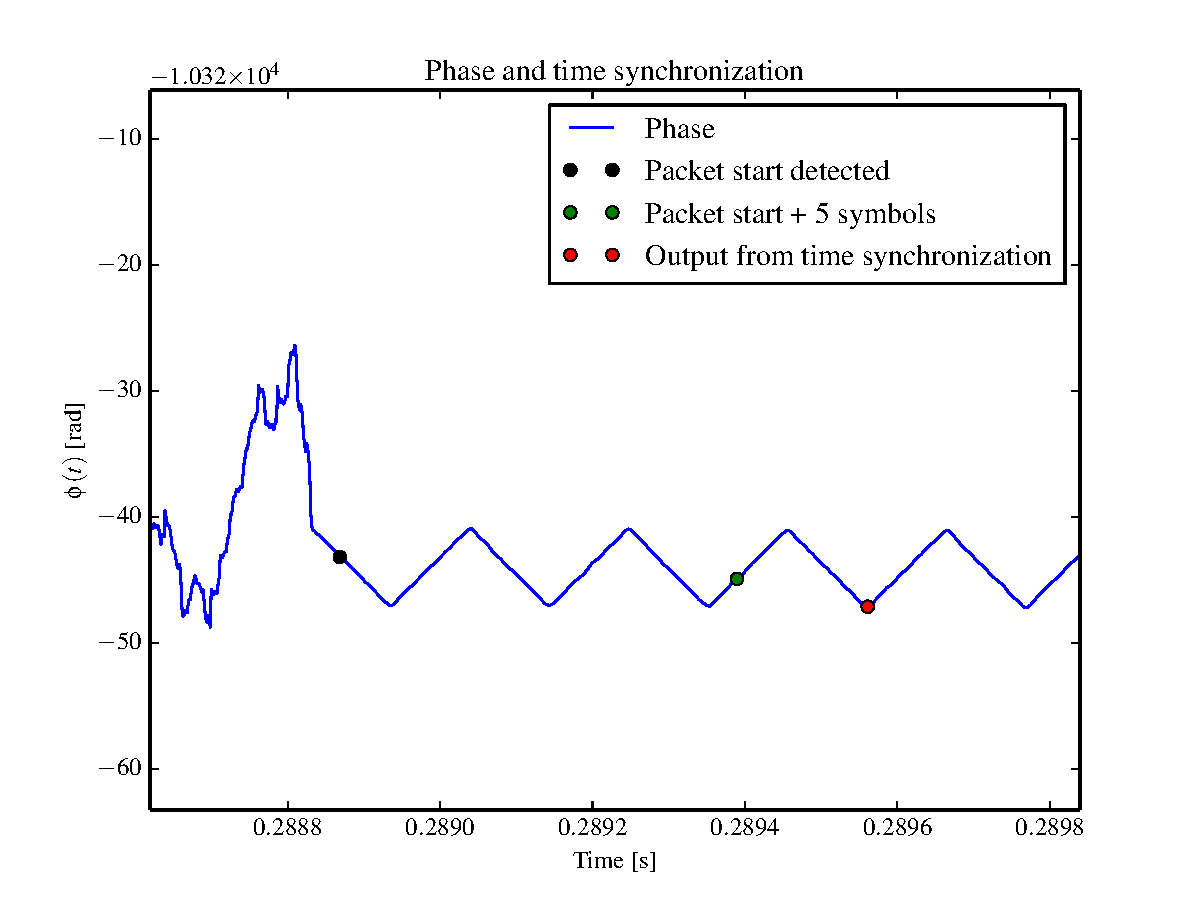
\includegraphics[width=0.8\textwidth]{img/time_sync_test}
    \end{center}
\end{frame}
